\documentclass[]{article} % A4 paper and 11pt font size
\usepackage[final]{pdfpages}
\usepackage[utf8]{inputenc}
\usepackage{amsmath,amsfonts,amsthm} % Math packages
\usepackage{outline}
\usepackage{makeidx}
\usepackage[gen]{eurosym}
\usepackage{graphicx}
\usepackage[portuguese]{babel} % Para termos legendas em português
\usepackage{pmgraph}
\usepackage[T1]{fontenc}
\usepackage[normalem]{ulem}
%\usepackage{undertilde}
%\usepackage{amssymb}
\usepackage{setspace}
\usepackage{indentfirst}
\usepackage{wrapfig}
\usepackage{mathtools}
\usepackage{amsmath} 
\usepackage{lipsum}
\usepackage{blindtext}
\usepackage{chngcntr}
\usepackage{tabu}
\usepackage{float}
\usepackage{easytable}
\usepackage{physics}
\usepackage{caption}
\usepackage{listings}
\usepackage{adjustbox}
\usepackage{setspace}
\usepackage{subfig}
\renewcommand{\baselinestretch}{1.5}
\counterwithin*{section}{part}
%% \setcounter{section}{1} % Começa a numeracao das sections por 2
\usepackage[resetlabels,labeled]{multibib}

%--------------------Make usable space all of page
\setlength{\parindent}{0.5cm}
\setlength{\oddsidemargin}{0in}
\setlength{\evensidemargin}{0in}
\setlength{\topmargin}{0in}
\setlength{\headsep}{-.25in}
\setlength{\textwidth}{6.5in}
\setlength{\textheight}{8.5in}
%--------------------Indention
\numberwithin{equation}{section} % Number equations within sections (i.e. 1.1, 1.2, 2.1, 2.2 instead of 1, 2, 3, 4)
\numberwithin{figure}{section} % Number figures within sections (i.e. 1.1, 1.2, 2.1, 2.2 instead of 1, 2, 3, 4)
\numberwithin{table}{section} % Number tables within sections (i.e. 1.1, 1.2, 2.1, 2.2 instead of 1, 2, 3, 4)
%---------------------
\newcommand{\horrule}[1]{\rule{\linewidth}{#1}} % Create horizontal rule command with 1 argument of height
\DeclareMathAccent{\wtilde}{\mathord}{largesymbols}{"65}

\newtheorem{theorem}{Teorema}
\newcommand{\euler}{e}
\newcommand{\im}{j}

\begin{document}
\begin{titlepage}
\begin{center}
\begin{figure}
\begin{flushleft}

\includegraphics[height=2.5cm]{./IST_logo.png}\\[2cm]
\end{flushleft}
\end{figure}
\title{Relatório Projeto STel}
\huge \textsc{Sistemas de Telecomunicações}\\[0.2cm]
\Large \textsc{2º Semestre 201/2019}\\[0.2cm]
\normalsize \textsc{MEEC\\[1cm]}
\horrule{1pt}\\[0cm]
\huge \textbf{PROJECTO DE UMA LIGAÇÂO POR FEIXES HERTEZIANOS}  % The assignment title
\horrule{1pt}\\[1cm]
\end{center}
\begin{center}
\large
Docentes : \\[1cm]
\end{center}
\begin{flushleft}
\Large \textbf{Group:}\\[4pt]
\large
-- João Filipe, Nº 76481; \\
-- Simão Valente, Nº 78089.\\[1.5cm]
\end{flushleft}
\centering
\Large
Lisboa, junho 2018
\thispagestyle{empty}
\end{titlepage}
\tableofcontents

\pagebreak
\section{Introdução}
O presente trabalho tem como objetivo elaborar um projeto de uma ligação bidirecional de feixes hertzianos digitais entre Montijo e Fontanelas para um sinal PDH/E-2 (8 Mbit/s) que suporta tráfego telefónico correspondente a um máximo de 120 canais telefónicos e que garanta as especificações ITU-R. Deste modo torna-se necessário a análise de diversas possibilidades no que concerne aos percursos mais adequados, à possível utilização de repetidores (ativos ou passivos), as frequências a utilizar, dimensão e altura das antenas, entre outros, tudo com o propósito de encontrar a solução mais económica para o custo de uma chamada bidirecional com a duração de 3 minutos.

De modo a cumprir dos objetivos, foram utilizadas ferramentas específicas, nomeadamente o script \textit{Feixer} do programa \textit{Mathematica}, que permite a verificação das cláusulas ITU-R e o cálculo de parâmetros essenciais à ligação, um link do \textit{Google Maps} que possibilita a obtenção do perfil da ligação e o \textit{Google Earth} permite retirar a orientação da antena.

\subsection{Especificações do projeto}
Para a realização do projeto foram-nos atribuídas as seguintes especificações:
\begin{itemize}
\item Valor máximo para a potência do emissor dado por \textit{$p_{m}=\frac{p_{0}}{f^b}$} com \textit{$p_{m}$} em W, \textit{f} em GHz, \textit{$p_{0}$}=7 e \textit{b}=1.2;
\item Factor do ruído no receptor dado por \textit{F=$F_{0}$+a*f} com \textit{F} em dB, \textit{f} em GHz,\textit{$F_{0}$}=7 e \textit{a}=0.1;
\item Determinação da banda de frequência óptima de entre as previstas pela ITU-R para os serviços pretendidos com as restrições da ANACOM;
\item Encargos de exploração anuais de 0.15 do custo inicial;
\item Encargos nulos com terrenos e direitos de passagem;
\item Taxa de utilização anual de acordo com o definido pela ANACOM;
\item Duração do projeto de 25 anos;
\item Tráfego médio por canal telefónico igual a (0.2+0.02*$t_{i[anos]}$) Erlang;
\item Taxa interna de retorno (a preços constantes) de 10%;
\item Taxa de inflação de 3%.
\end{itemize}


\section{Parâmetros da ligação}
Nesta secção são analisados os diversos parâmetros escolhidos para configurar a ligação, bem como a justificação do motivo para a escolha dos mesmos.
\subsection{Plano de Frequências }
Sendo a frequência de trabalho um dos principais parâmetros a determinar, foi consultado o \textit{website} da ANACOM através do \textit{link} fornecido no enunciado do projeto. A ANACOM é a entidade responsável em Portugal para regulação do espetro disponível para as ligações de ponto-a-ponto bidirecionais onde se averiguaram quais as frequências e larguras de banda previstas pela ITU-R. Assim sendo, das frequências disponíveis para as ligações ponto-a-ponto retiramos as que consideramos ser apropriadas para o nosso projeto,que se encontram na tabela \ref{freqUsar}.

\begin{table}[H]
\centering
\begin{tabular}{|c|c|}
\hline
Frequências (GHz) & Espaçamento (MHz)\\
\hline
2 & 1.75, 3.5, 7, 14\\
6 & 20, 29.65, 40\\
7 & 1.75, 3.5, 7, 14, 28, 56\\
8 & 29.65\\
11 & 40\\
13 & 3.5, 7, 14, 28, 56\\
15 & 3.5, 7, 14\\
18 & 3.5, 7.5, 13.75, 27.5, 55\\
\hline
\end{tabular}
\caption{Frequências utilizadas.}
\label{freqUsar}
\end{table}

É importante referir que não foram tomadas em consideração frequências superiores a 18GHz devido à elevada atenuação causada pela chuva, daí não compensar a sua utilização.

Para determinar a largura de banda da radiofrequência foi utilizada a seguinte fórmula:

\begin{equation}
\centering
f_{s}=\frac{LB}{1+\alpha}
\end{equation}
\begin{itemize}
\item LB é o espaçamento teórico em MHz;
\item $\alpha$ é o fator de excesso de banda, inicialmente considerado 0.1.
\end{itemize} 
No caso da determinação do número de níveis por palavra a utilizar foi tomada em consideração a formula:

\begin{equation}
\centering
M=2^\frac{f_{b}}{f_{s}}
\end{equation}

\begin{itemize}
\item $f_{b}$ a representar o débito binário. 
\end{itemize}

\begin{table}[H]
\centering
\begin{tabular}{|c|c|c|c|}
\hline
LB (MHz) & $f_{s}$ & M &  Modulação\\
\hline
1.75 & 1.591 & 32.640 & 64-QAM\\
3.5 & 3.182 & 5.713 & 8-PSK\\
7 & 6.364 & 2.390 & 4-PSK\\
7.5 & 6.818 & 2.255 & 4-PSK\\
13.75 & 12.5 & 1.558 & 2-PSK\\
14 & 12.727 & 1.546 & 2-PSK\\
20 & 18.182 & 1.357 & 2-PSK\\
27.5 & 25 & 1.248 & 2-PSK\\
28 & 25.455 & 1.243 & 2-PSK\\
29.65 & 26.955 & 1.228 & 2-PSK\\
40 & 36.364 & 1.165 & 2-PSK\\
55 & 50 & 1.117 & 2-PSK\\
56 & 50.909 & 1.115 & 2-PSK\\
\hline
\end{tabular}
\caption{Modulações possíveis para um débito binário de 8 Mbit/s.}
\label{modulação}
\end{table}

Com os níveis de modulação a utilizar definidos é necessário determinar o valor efetivo do fator de excesso de banda real que poderá qualquer valor entre 0.1 e 0.5 inclusive. No que diz respeito a modulação é sabido que o desempenho do M-QAM, para o mesmo número de níveis por palavra, é igual ou superior ao do M-PSK, nomeadamente para valores elevados de M. Ainda assim o PSK é utilizado devido a sua simplicidade. Segundo as especificações do projeto os tipos de modulações possíveis restringem-se a 2-PSK, 4-PSK, 8-PSK, 16-QAM, 64-QAM e 256-QAM.

No que concerne as larguras de banda dentro da mesma frequência e que utilizam a mesma modulação, foram escolhidas apenas as de valor inferior de modo a evitar o não aproveitamento dessa largura de banda.
Seguem na tabela \ref{fatorExcessoBanda} os valores a analisar.

\begin{table}[H]
\centering
\begin{tabular}{|c|c|c|c|c|}
\hline
LB (MHz) & Modulação & M & $f_{s}$ & $\alpha$ \\
\hline
1.75 & 64-QAM & 64 & 1.33 & 0.31\\
3.5 & 8-PSK & 8	& 2.66 & 0.31\\
7 & 4-PSK & 4 & 4 & 0.75\\
7.5 & 4-PSK & 4 & 4 & 0.875\\
13.75 & 2-PSK & 2 & 8 & 0.719\\
14 & 2-PSK & 2 & 8 & 0.75\\
20 & 2-PSK & 2 & 8 & 1.5\\
27.5 & 2-PSK & 2 & 8 & 2.44\\
28 & 2-PSK & 2 & 8 & 2.5\\
29.65 & 2-PSK & 2 & 8 & 2.71\\
40 & 2-PSK & 2 & 8 & 4\\
55 & 2-PSK & 2 & 8 & 5.88\\
56 & 2-PSK & 2 & 8 & 6\\
\hline
\end{tabular}
\caption{Fator de excesso de banda.}
\label{fatorExcessoBanda}
\end{table}
Importa realçar que para os valores de $\alpha$ que ultrapassam o limite máximo permitido (0.5) serão considerados como 0.5, ou seja, a partir de LB=7MHz até 56MHz.

\subsection{Atenuações e indisponibilidade}
Na realização do projeto foram tidas em conta diversas atenuações determinadas através do \textit{Feixer}, nomeadamente atenuação em espaço livre, atenuação do obstáculo, reflexões do terreno, atenuação atmosférica, atenuação devida aos hidrometeoritos (polarização horizontal) e a atenuação devida aos guias (10 metros de comprimento).

Relativamente a indisponibilidade máxima foram atribuídos os seguintes parâmetros: 10\% devido á chuva, 40\% devido ao equipamento e 50\% devido outras causas.


\subsection{Análise da ligação}
Previamente à ligação entre o emissor e o recetor foi necessário ter em consideração para a colocação das antenas os seguintes aspetos: altitude do local, acessibilidade, distância inferior a 1Km do centro da localidade, evitar locais históricos ou com interesse turístico e posicionamento de forma a evitar reflexões que pudessem vir a interferir com o sinal emitido. 


Deste modo foi possível obter, através do \textit{Google Earth} as coordenadas da posição das antenas:
\begin{table}[H]
\centering
\begin{tabular}{|c|c|c|c|}
\hline
Localização & Latitute & Longitude & Cota (m)\\
\hline
Montijo & 38º42'43''N & 8º58'10''W & 16\\
Fontanelas & 38º50'55''N & 9º26'21''W & 128\\
\hline
\end{tabular}
\caption{Coordenadas das posições das antenas.}
\label{coord}
\end{table}

Numa primeira fase verificou-se o perfil da ligação direta Montijo-Fontanelas apresentado na figura abaixo.
\begin{figure}[H]
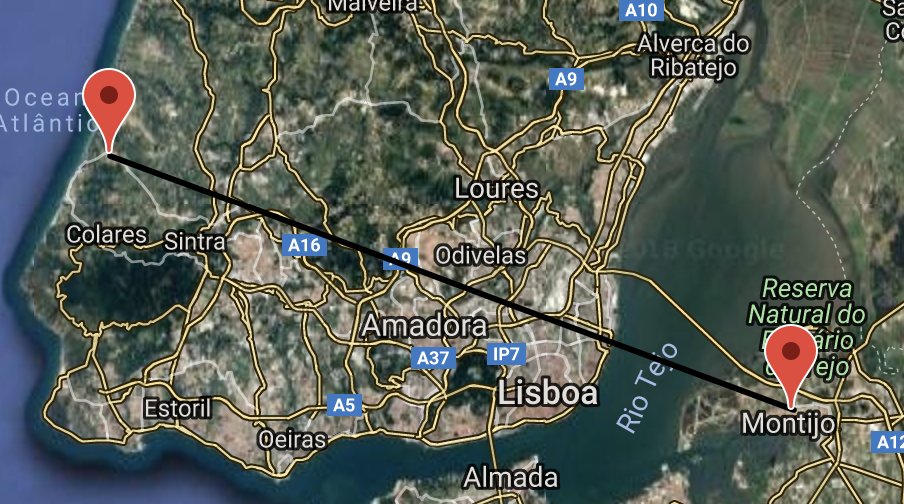
\includegraphics[scale=0.5]{Ligac_a_o_direta_Fontanelas-Montijo.png}
\centering
\caption{Ligação em linha reta entre Montijo e Fontanelas.}
\end{figure}
\begin{figure}[H]
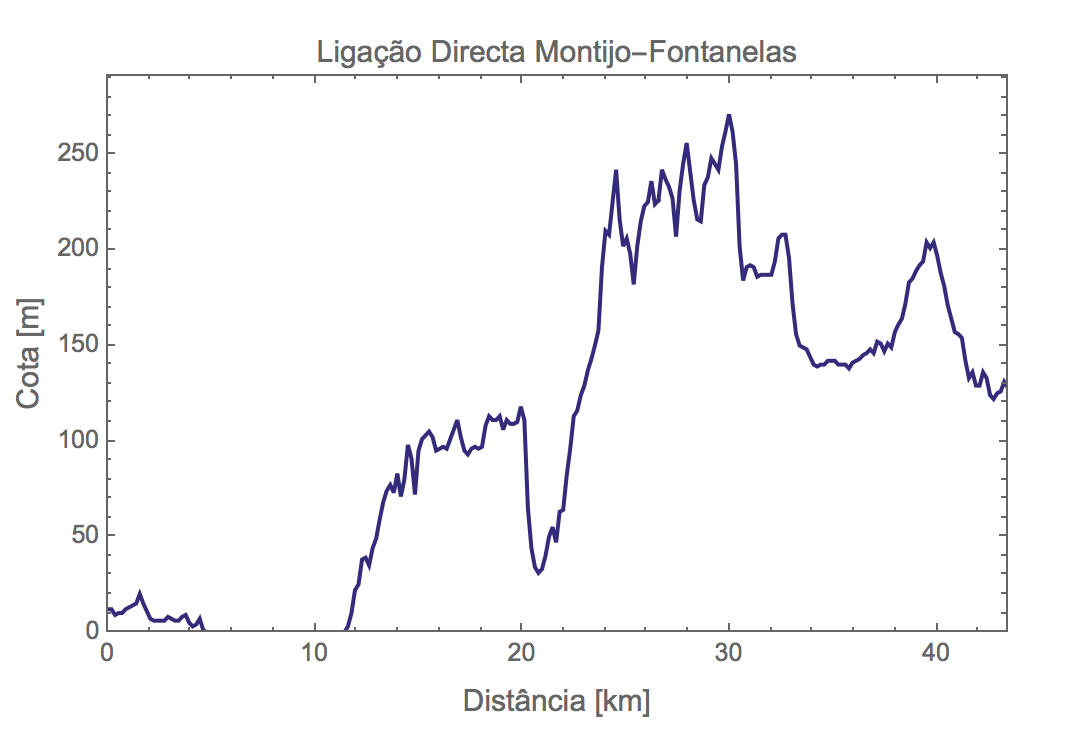
\includegraphics[scale=0.5]{perfil_d.png}
\centering
\caption{Perfil para uma ligação em linha reta entre Montijo e Fontanelas.}
\end{figure}

Pela análise do perfil é possível averiguar a existência de obstáculos na ligação direta, assim como a necessidade de mais que 1 repetidor para estabelecer a ligação entre o emissor e o recetor. Deste modo procedeu-se a uma análise do terreno para melhorar o perfil e tentar evitar a colocação de mais de um repetidor ou a colocação de um repetidor com um mastro superior a 30 metros\footnote{Devido ao elevado preço do mastro para alturas superiores a 30 metros.}. Resultando numa percurso alternativo entre o emissor e o recetor, como se apresenta nas figuras abaixo.

\begin{figure}[H]
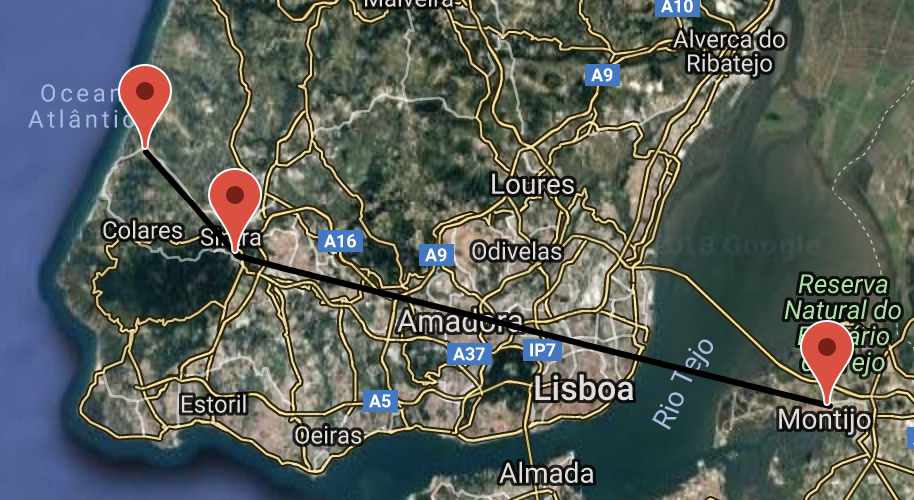
\includegraphics[scale=0.5]{ligacao_m-s-f.png}
\centering
\caption{Ligação não em linha reta entre Montijo e Fontanelas.}
\end{figure}
\begin{figure}[H]
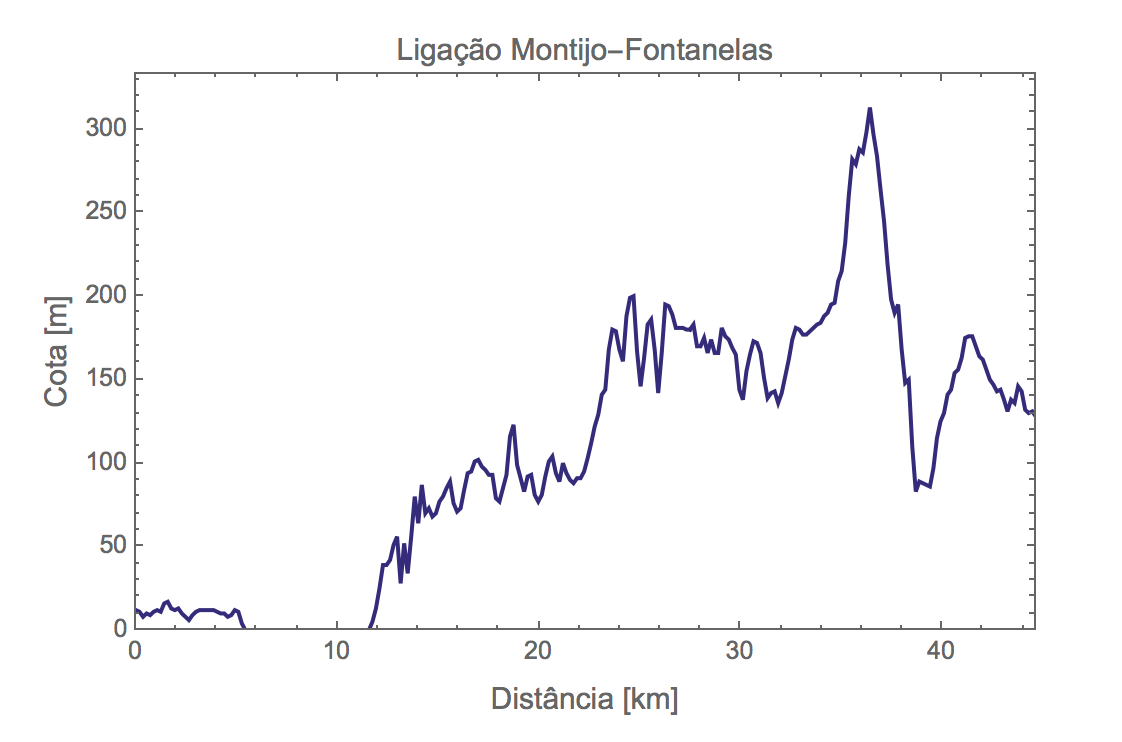
\includegraphics[scale=0.5]{perfil.png}
\centering
\caption{Perfil para uma ligação não em linha reta entre Montijo e Fontanelas.}
\end{figure}

Com este novo perfil, verifica-se que a colocação de apenas um repetidor a uma altura não superior a 30 metros permitirá a ligação entre Montijo e Fontanelas. Assim utilizou-se este perfil para a análise da ligação no \textit{Feixer}, obtendo-se os seguintes Elipsóides de Fresnel.
Assim a distância determinada no \textit{Feixer} entre emissor e recetor é de 44.632 Km, sendo que os terminais não se encontram em linha de vista devido ao obstáculo natural que se encontra à distância de 36.406Km do Montijo. Deste modo torna-se necessário determinar uma alternativa que possibilite a ligação, existindo mais que uma, será tida em conta a que apresentar um menor custo.
\begin{figure}[H]
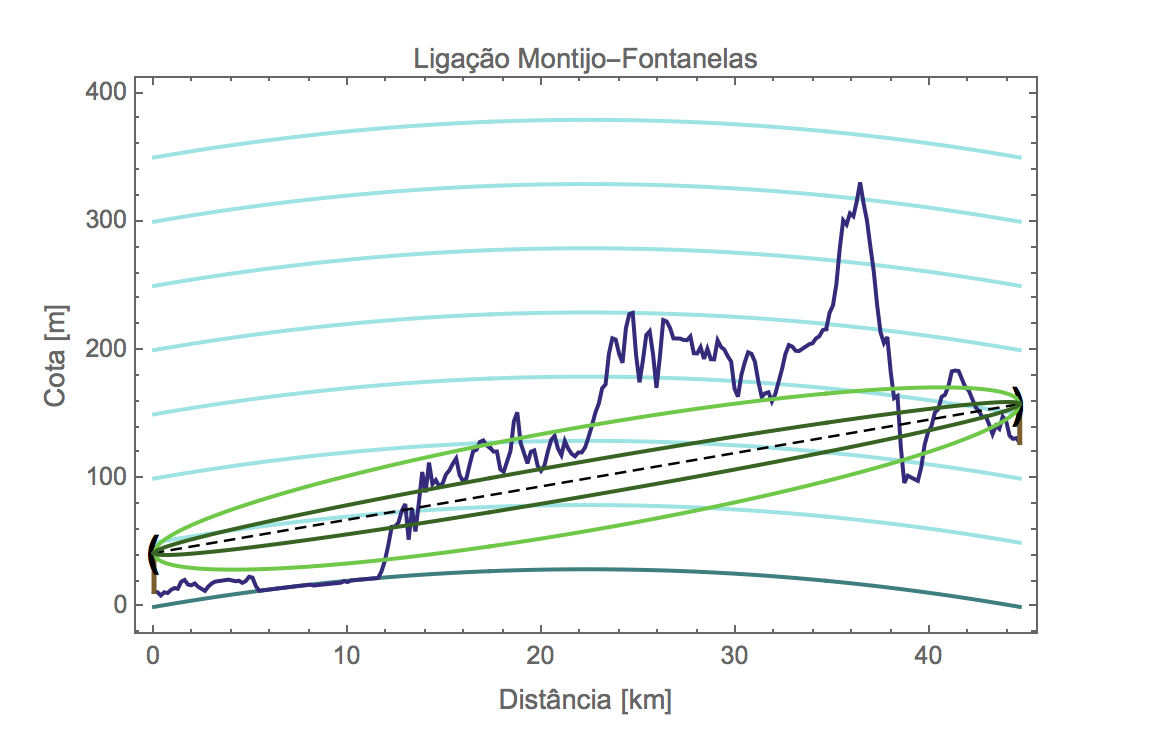
\includegraphics[scale=0.5]{fresnel_dir.png}
\centering
\caption{Representação do 1º Elipsóide de Fresnel para a ligação direta entre Montijo e Fontanelas.}
\end{figure}

\subsection{Ligação com recurso a um repetidor passivo no percurso alternativo}

Com o auxílio do \textit{Feixer} é possível posicionar um repetidor, neste caso, costas com costas no local do obstáculo identificado a 36.406Km do Montijo. As coordenadas do repetidor encontram-se na seguinte tabela:
\begin{table}[H]
\centering
\begin{tabular}{|c|c|c|c|}
\hline
Localização & Latitude & Longitude & Cota(m)\\
\hline
Serra de Sintra & 38º47'33'' N & 9º 22' 38''W & 313\\
\hline
\end{tabular}
\caption{Coordenadas do repetidor retiradas a partir do \textit{Google Earth}.}
\label{coord_rep}
\end{table}
Foram introduzidos, numa fase inicial, os seguintes parâmetros no \textit{script Feixer}, possíveis de serem alterados de acordo com a melhor solução:

\begin{table}[H]
\centering
\begin{tabular}{|c|c|}
\hline
Parâmetro & Valor\\
\hline
Rendimento do Repetidor & 1\\
Diâmetro da antena de emissão[m] & 4.5\\
Diâmetro da antena de receção[m] & 4.5\\
Rendimento de abertura das antenas de emissão e receção & 0.5\\
Diâmetro da antena de emissão do repetidor[m] & 4.5\\
Diâmetro da antena de receção do repetidor[m] & 4.5\\
Folga dos guias de onde [m] & 10 \\
Área efetiva do repetidor[$m^2$] & 7.95216\\
Altura do mastro de emissão do repetidor & 6\\
Altura do mastro de receção do repetidor & 15\\
Altura do mastro da antena de emissão & 30\\
Altura do mastro da antena de receção & 30\\
\hline
\end{tabular}
\caption{Características da ligação introduzidas no \textit{Feixer}.}
\end{table}
A área efetiva do repetidor passivo é determinada pela expressão 
\begin{equation}
a_{ef}=\pi(\frac{D}{2})^2\eta_{a} [m^2]
\end{equation}
sendo que:
\begin{itemize}
\item D -  diâmetro da antena de emissão/receção do repetidor;
\item $\eta_{a}$ - rendimento da antena de emissão/receção, neste caso tomou o valor de 0.5.
\end{itemize}
O 1º elipsóide de Fresnel para a ligação com repetidor passivo encontra-se na figura \ref{ligacaoComRep}.
\begin{figure}[H]
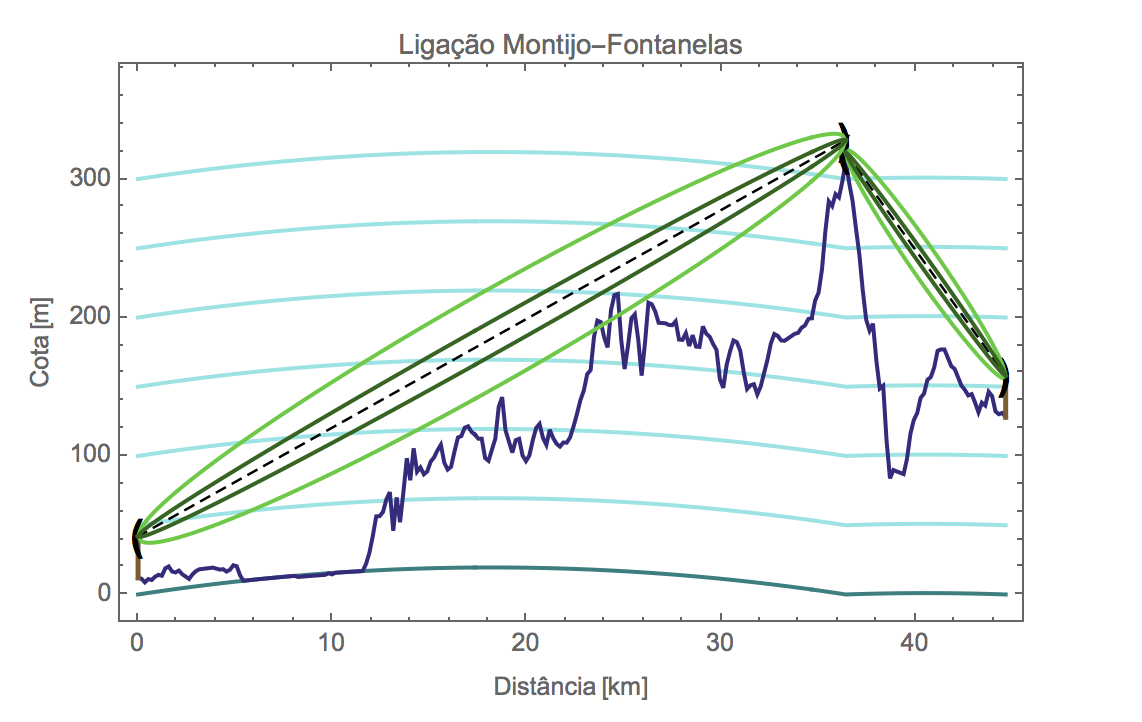
\includegraphics[scale=0.5]{elipsoide_f.png}
\centering
\caption{Ligação com repetidor Montijo-Fontanelas.}
\label{ligacaoComRep}
\end{figure}

É de salientar que a localização do repetidor se encontra na zona próxima do recetor e que se verificou valores da relação $\frac{p_{s}}{p_{d}}$ inferior da -10dB para todas as frequências, deste modo evitam-se os problemas com as reflexões no terreno, podendo utilizar estas frequência para o cumprimento das normas da ITU-R. Ainda assim apresenta-se na figura \ref{reflexoes} as reflexões no terreno consideradas pelo \textit{Feixer} para a frequência de 2GHz, sendo que para esta frequência verificasse a menor relação $\frac{p_{s}}{p_{d}}$.

Para ser possível garantir as cláusulas ITU-R é necessário que para uma determinada frequência, largura de banda e modulação se cumpra a condição $(\frac{C}{N})_{CIP} - (\frac{C}{N})_{NECmin}> 3 $dB, em que:
\begin{itemize}
\item $\frac{C}{N}_{CIP}$ $\Rightarrow$ Relação sinal - ruído da ligação em condições ideais de propagação;
\item $\frac{C}{N}_{NECmin}$ $\Rightarrow$ Relação sinal - ruído mínima necessária para cumprir as cláusulas.
\end{itemize}

Deste modo apresentam-se os resultado na tabela \ref{margemLigacao}, onde se verifica que não existe qualquer frequência que cumpra a condição acima mencionada, o que implica a necessidade de projeção de um repetidor ativo.  
\begin{table}[H]
\centering
\begin{tabular}{|c|c|c|c|c|c|}
\hline
Frequências [GHz] & LB [MHz] & Tipo de Modulação & $\alpha$ & Margem de Ligação [dB] \\
\hline
 & 1.75 & 64-QAM & 0.31 & -32.1773\\
2 & 3.5 & 8-PSK & 0.31 & -23.6475\\
 & 7 & 4-PSK & 0.5 & -20.1595\\
\hline
 6 & 20 & 2-PSK & 0.5 & -13.6672\\
\hline
 & 1.75 & 64-QAM & 0.31 & -24.9565\\
7 & 3.5 & 8-PSK & 0.31 & -16.4175\\
 &7 & 4-PSK & 0.5 & -12.9031\\
\hline
8 & 29.65 & 2-PSK & 0.5 & -14.9241\\
\hline
11 & 40 & 2-PSK & 0.5 & -15.1301\\
\hline
13 & 3.5 & 8-PSK & 0.31 & -19.1322\\
& 7 & 4-PSK & 0.5 & -15.5991\\
\hline
15 & 3.5 & 8-PSK & 0.31 & -22.8457\\
 & 7 & 4-PSK & 0.5 & -19.6259\\
\hline
18 & 3.5 & 8-PSK & 0.31 & -47.8929\\
& 7.5 & 4-PSK & 0.5 & -44.6722\\ 
\hline
\end{tabular}
\caption{Margem de ligação para as diferentes frequências e larguras de banda.}
\label{margemLigacao}
\end{table}

\subsection{Ligação com recurso a um repetidor ativo no percurso alternativo}

Poderiam-se ter utilizado outras soluções como a igualação ou diversidade no espaço através da colocação de mais antenas recetoras, mas o enunciado restringia estas soluções. Para realizar o estudo da ligação com recurso a um repetidor ativo consideraram-se dois troços: Montijo-Serra de Sintra e Serra de Sintra-Fontanelas. Numa primeira fase considerou-se o troço de maior extensão, neste caso, Montijo-Serra de Sintra, para determinar a frequência ótima para a ligação, sendo que, para o troço de menor dimensão utilizou-se essa frequência determinada.

Sendo o objetivo do projeto determinar a ligação com o menor custo possível, consideraram-se alguns parâmetros diferentes face à ligação com o repetidor passivo, nomeadamente:
\begin{itemize}
\item Troço 2 : Serra de Sintra - Fontanelas
\begin{itemize}
\item Altura do mastro da antena de emissão [m] $\rightarrow$ 25;
\item Altura do mastro da antena de receção [m] $\rightarrow$ 20;
\end{itemize}
\end{itemize}
Ainda se analisaram diversas possibilidades para o diâmetro menores na antena e no repetidor no troço 2, no entanto as reflexões para os 2 GHz eram significativas, então optou-se por não alterar os diâmetros e considerar a frequência de 2 GHz para os cálculos.
Relativamente aos perfis de ambos os troços, podem-se verificar nas figuras \ref{perfil1} e \ref{perfil2}, que não existem quaisquer obstáculos à ligação.

Relativamente as reflexões no terreno verificou-se individualmente para ambos os troços que estas são em tudo semelhantes às determinadas anteriormente com o perfil completo\footnote{Por completo entenda-se sem troços, ou seja, perfil Montijo-Fontanelas.}. Assim sendo consideraram-se as reflexões no terreno desprezáveis para a projeção da ligação.

Verificaram-se as diversas frequências e larguras de banda para o troço 1 e os resultados encontram-se na tabela \ref{reflexoes1}, onde se verifica que, exceto os 18 GHz, todas as frequências cumprem a condição da margem de ligação > 3 dB. 
\begin{table}[H]
\centering
\begin{tabular}{|c|c|c|c|c|}
\hline
Frequências [GHz] & LB [MHz] & Tipo de Modulação & $\alpha$ & Margem de Ligação [dB] \\
\hline
 & 1.75 & 64-QAM & 0.31 & 12.4002\\
2 & 3.5 & 8-PSK & 0.31 & 20.929 \\
 & 7 & 4-PSK & 0.5 & 24.418\\
\hline
 6 & 20 & 2-PSK & 0.5 & 20.7033\\
\hline
 & 1.75 & 64-QAM & 0.31 & 8.09423\\
7 & 3.5 & 8-PSK & 0.31 & 16.6332\\
 &7 & 4-PSK & 0.5 & 20.1476\\
\hline
8 & 29.65 & 2-PSK & 0.5 & 18.6513\\
\hline
11 & 40 & 2-PSK & 0.5 & 14.1184\\
\hline
13 & 3.5 & 8-PSK & 0.31 & 8.77458\\
& 7 & 4-PSK & 0.5 & 12.3077\\
\hline
15 & 3.5 & 8-PSK & 0.31 & 4.40697\\
 & 7 & 4-PSK & 0.5 & 7.94437\\
\hline
18 & 3.5 & 8-PSK & 0.31 & -17.4602\\
& 7.5 & 4-PSK & 0.5 & -14.2395\\ 
\hline
\end{tabular}
\caption{Margem de ligação para o troço 1.}
\label{reflexoes1}
\end{table}
Foi necessário realizar a mesma verificação das cláusulas para o troço 2, mas neste caso desprezou-se a frequência de 18 GHz, por não respeitar as cláusulas ITU-R no Montijo-Serra de Sintra. Os resultados para a margem apresentam-se na tabela \ref{reflexoes2}. De acordo com os resultados, a ligação respeita a cláusula com uma margem bastante grande, ou seja, a única maneira possível para reduzir esta margem seria através da redução do diâmetro das antenas de emissão, receção e do repetidor ativo, uma fez que foram testadas várias alturas para os mastros das antenas sendo as apresentadas as menores que garantem uma ligação sem obstáculos, nem reflexões consideráveis.
Uma vez que existem diversas possibilidades, foram desprezadas o conjunto de frequências [6,8,11] por apresentarem uma largura de banda muito grande, restando as frequências [2,7,13,15] para analisar.  
\begin{table}[H]
\centering
\begin{tabular}{|c|c|c|c|c|}
\hline
Frequências [GHz] & LB [MHz] & Tipo de Modulação & $\alpha$ & Margem de Ligação [dB] \\
\hline
 & 1.75 & 64-QAM & 0.31 & 51.7625\\
2 & 3.5 & 8-PSK & 0.31 & 60.2866\\
 & 7 & 4-PSK & 0.5 & 63.7586\\
\hline
 6 & 20 & 2-PSK & 0.5 & 60.9548\\
\hline
 & 1.75 & 64-QAM & 0.31 & 48.6677\\
7 & 3.5 & 8-PSK & 0.31 & 57.1918\\
 &7 & 4-PSK & 0.5 & 60.6639\\
\hline
8 & 29.65 & 2-PSK & 0.5 & 59.4535\\
\hline
11 & 40 & 2-PSK & 0.5 & 56.0951\\
\hline
13 & 3.5 & 8-PSK & 0.31 & 51.5688\\
& 7 & 4-PSK & 0.5 & 55.041 \\
\hline
15 & 3.5 & 8-PSK & 0.31 & 48.5089\\
 & 7 & 4-PSK & 0.5 & 51.9811\\
\hline
\end{tabular}
\caption{Margem de ligação para o troço 2.}
\label{reflexoes2}

\end{table}

\subsection{Cálculo dos ângulos de fogo e azimutes}
A representação no terreno dos ângulos de fogo pode ser verificada na figura \ref{fogo}.

\begin{figure}[H]
\centering
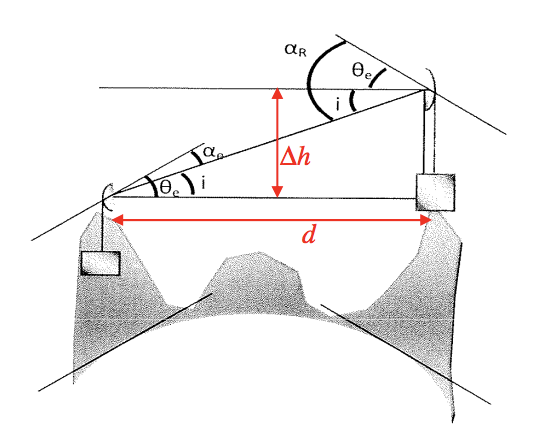
\includegraphics[scale=0.8]{angulosfogo.png}
\caption{Ilustração para a determinação dos ângulos de fogo.}
\label{fogo}
\end{figure}

Com base na figura acima ilustrada, pode-se considerar:
\begin{equation}
\centering
\alpha_{E} = \theta_{E}-i
\end{equation}
\begin{equation}
\centering
\alpha_{R} = \theta_{E}+i
\end{equation}
Sendo que:
\begin{equation}
i = tan^{-1}(\frac{\Delta h}{d})
\end{equation}
\begin{equation}
\theta_{E} = tan^{-1}(\frac{d/2}{r_{e}})
\end{equation}

$r_{e} \rightarrow$ raio equivalente da Terra.

Foram considerados os seguintes dados e calculados dos ângulos de fogo:
\begin{table}[H]
\centering
\begin{tabular}{|c|c|c|}
\hline
Parâmetro & Troço 1: Montijo-Serra de Sintra & Troço 2: Serra de Sintra-Fontanelas\\
\hline
$r_{e}$ [m] & 8493330 & 8493330\\
$h_{MastroEmissao/RepetidorAtivo}$ [m] & 30 & 25\\
$h_{MastroRepetidorAtivo/Rececao}$ [m] & 30 & 20\\
d [m] & 36406 & 8632\\
$\Delta h$ [m] & 343-46=297 & 338-148=190\\
i [º]& 0.4674 & 1.2278\\
$\theta_{E}$ [º] & 0.12298 & 0.029116\\
$\alpha_{E}$ [º] & -0.34461 & -1.19868\\
$\alpha_{R}$ [º] & 0.59038 & 1.25692\\
\hline
\end{tabular}
\caption{Ângulos de fogo}
\label{A_fogo}
\end{table}

Os azimutes são determinados com base nas coordenadas apresentadas nas tabelas \ref{coord} e \ref{coord_rep}, convertendo as unidades para graus decimais e baseados nas seguintes equações:

\begin{equation}
y=arctan(cot(\frac{|g_{R}-g_{E}|}{2})\frac{sin(\frac{t_{R}-t_{E}}{2})}{cos(\frac
{t_{R}+t_{E}}{2})})+arctan(cot(\frac{|g_{R}-g_{E}|}{2})\frac{cos(\frac{t_{R}-t_{E}}{2})}{sin(\frac
{t_{R}+t_{E}}{2})}
\end{equation}
\begin{equation}
x=arctan(cot(\frac{|g_{R}-g_{E}|}{2})\frac{cos(\frac{t_{R}-t_{E}}{2})}{sin(\frac
{t_{R}+t_{E}}{2})})+arctan(cot(\frac{|g_{R}-g_{E}|}{2})\frac{sin(\frac{t_{R}-t_{E}}{2})}{cos(\frac
{t_{R}+t_{E}}{2})}
\end{equation}
Os troços considerados encontram-se nas seguintes figuras:

\begin{figure}[!tbp]
\subfloat[Montijo-Serra de Sintra]{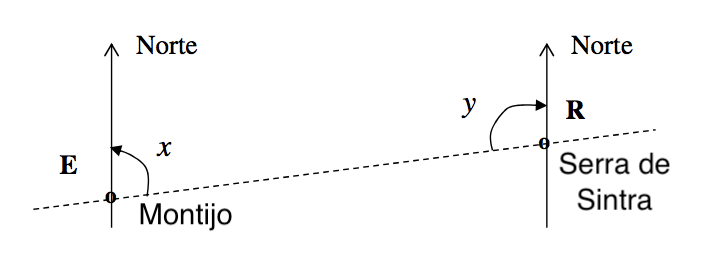
\includegraphics[width=0.5\textwidth]{az_m_s.png}}
\subfloat[Serra de Sintra-Fontanelas]{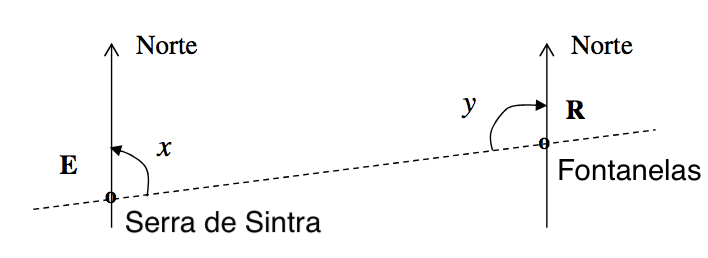
\includegraphics[width=0.5\textwidth]{az_s_f.png}}
\caption{Troços considerados para determinação de azimute }
\end{figure}
Com base nos troços definidos, os azimutes encontram-se representados na tabela \ref{azimutes}.

\begin{table}[H]
\centering
\begin{tabular}{|c|c|}
\hline
Sentido & Azimute [º]\\
\hline
Montijo-Serra de Sintra & 58.3155\\
Serra de Sintra-Montijo & 258.7038\\
Serra de Sintra-Fontanelas & -137.8252\\
Fontanelas-Serra de Sintra & 402.1215\\
\hline
\end{tabular}
\caption{Azimutes}
\label{azimutes}
\end{table}

\section{Análise de Custos}
Com as características mais relevantes da ligação determinadas é agora possível realizar o estudo do custo de uma chamada de 3 minutos para um período de 25 anos e assim determinar qual a frequência que minimiza o custo da chamada.

\subsection{Taxa de utilização anual}
Existe um preço a pagar pela utilização do espetro eletromagnético e como tal, apresenta-se uma tabela que explana os custos para as frequências em estudo, a qual foi parcialmente retirada do \textit{website} da ANACOM.

\begin{table}[H]
\centering
\begin{tabular}{|c|ccc|}
\hline
Faixa de Frequências [GHz] & 1-3 & 4-11 & 12-15\\
\hline
Comprimento mínimo da ligação $L_{min}$ & n.a & 10 km &5 km\\
\hline
Taxa por MHz [euros] & 48.5$\sqrt[2]{L}$ & 57.5$\sqrt[2]{L}$& 30.5$\sqrt[2]{L}$\\
\hline
Código da taxa & 143101 & 143102 & 143103\\
\hline
\end{tabular}
\caption{Taxa aplicável por ligação hertziana bidirecional e por canal designado.}
\label{taxa}
\end{table}
Sendo L a distância da ligação hertziana em quilómetros. 

De acordo com a tabela \ref{taxa} é possível determinar o custo de cada frequência e respetiva largura de banda ao ano\footnote{O custo foi determinado através do simulador fornecido no site da ANACOM para ligações bidirecionais com frequências da portadora superiores a 1 GHz, considerando apenas um canal bidirecional.}.
\begin{table}[H]
\centering
\begin{tabular}{|c|c|c|c|}
\hline
Frequência [GHz] & LB [MHz] & Custo anual [$\euro$]\\
\hline
 & 1.75 & 756.55\\
2 & 3.5 & 1 513.10\\
 & 7 & 3 026.21\\
 & 1.75 & 926.29\\
\hline
7 & 3.5 & 1 852.60\\
 & 7 & 3 705.20 \\
\hline
13 & 3.5 & 951.54\\
 & 7 & 3 1 903.08 \\
\hline
15 & 3.5 & 951.54\\
 & 7 & 1 903.08 \\
\hline
\end{tabular}
\caption{Custo anual para as diversas frequências.}
\label{custo_ano}
\end{table}
Com base na tabela apresentada verificasse que o menor custo anual corresponde à frequência de 2 GHz e uma LB=1.75 MHz. 

\subsection{Investimento Inicial}
Inicialmente é necessário considerar os custos associados aos materiais e equipamentos fundamentais para o projeto. Sendo assim, foram considerados os seguintes custos:
\begin{itemize}
\item Antenas parabólicas = 1000 + 75$D^3$	[D em metros]
\item Torres metálicas auto-suportadas = 4000 + 600h	[h em metros]
\item Guias de onde elípticos = 15(1+$\frac{10}{f})l_{guia}$	[$l_{guia}$ em metros; f em GHz]
\item Emissor + Recetor = 35 000 $\euro$
\item Abrigo e sistema de alimentação de energia = 60 000 $\euro$
\end{itemize}

\begin{table}[H]
\centering
\begin{tabular}{|c|cc|}
\hline
Descrição & Quantidade & Custo ($\euro$)\\
\hline
Antenas [D=4.5m] & 4 & 31337.5\\
Torres [h=30m] & 2 & 44000\\
Torre [h=25m] & 1 & 19000\\
Torre [h=20m] & 1 & 16000\\
Guias [l=10m;f=2GHz] & 4 & 3600 \\
Guias [l=10m;f=7GHz] & 4 & 1457.14 \\
Guias [l=10m;f=13GHz] & 4 & 1061.54 \\
Guias [l=10m;f=15GHz] & 4 & 1000 \\
Emissor + Recetor & 3 & 105000\\
Abrigo e sistema de alimentação de energia & 3 & 180000\\
\hline
Total & 2 GHz & 398937.5\\
 & 7 GHz & 396794.64\\
 & 13 GHz & 396399.04\\
 & 15 GHz & 396337.5\\
\hline
\end{tabular}
\caption{Custo do investimento inicial}
\label{custo_ini}
\end{table}

\subsection{Custos para o Utilizador, despesas e receitas}

As despesas anuais são dadas pela formula:
\begin{equation}
d_{t} = 0.15 \times d_{0} + TB_{LB/ano}
\end{equation}
Em que 0.15 $\times$ $d_{0}$ corresponde aos encargos de exploração anuais, dados por 15\% do investimento inicial calculado anteriormente, e $T_{LB/ano}$ refere-se à taxa de utilização anual (tabela \ref{taxa}). Sendo assim a despesa anual toma os valores:

\begin{table}[H]
\begin{tabular}{|c|c|c|c|c|}
\hline
Frequência [GHz] & 2 (LB=1.75MHz) & 7 (LB=3.5MHz) & 13 (LB=3.5MHz) & 15 (LB=3.5MHz) \\
\hline
$d_{t}$ & 60597.175 & 61372.096 & 60411.396 & 60402.165\\
\hline
\end{tabular}
\caption{Despesas anuais por frequência.}
\end{table}

Para um determinado ano \textit{t}, as receitas relativas ao tráfego telefónico são dadas por:
\begin{equation}
r_{t}=n \times T_{tel} \times N \times C_{3}
\end{equation}
 Em que \textit{n} corresponde ao número de canais telefónicos (120), \textit{$T_{tel}$} ao tráfego médio por canal telefónico no ano \textit{t}($T_{tel}$=0.2+0.02 $\times$ t), \textit{N} é o número de chamadas de 3 minutos num ano ($\frac{365.4 \times 24 \times 60}{3}$) e $C_{3}$ representa os custos de uma chamada de 3 minutos.
 
O custo de uma chamada de 3 minutos é dado por:
\begin{equation}
C_{3}= \frac{cte +0.15 \times d_{0} + TB_{LB/ano}}{n \times N \times T_{tel}}
\end{equation}
Para o valor residual ser nulo ao fim de 25 anos e considerando o \textit{cash overflow} constante, pode-se calcular o valor da constante, pela seguinte expressão:
\begin{equation}
cte = \frac{d_{0}}{\sum_{t=1}^{25}\frac{1}{(1+i)^t \times (1+tir)^t}}
\end{equation}

Considerou-se ainda a taxa de inflação \textit{i} de 3\% e a taxa interna de retorno \textit{tir} de 10\%.
De acordo com os dados apresentados e com o auxílio da ferramenta \textit{Excel}, obtiveram-se os custos associados a uma chamada de 3 minutos para o utilizador ao longo de 25 anos, representados na figura \ref{custo_user}.

\begin{figure}[H]
\centering
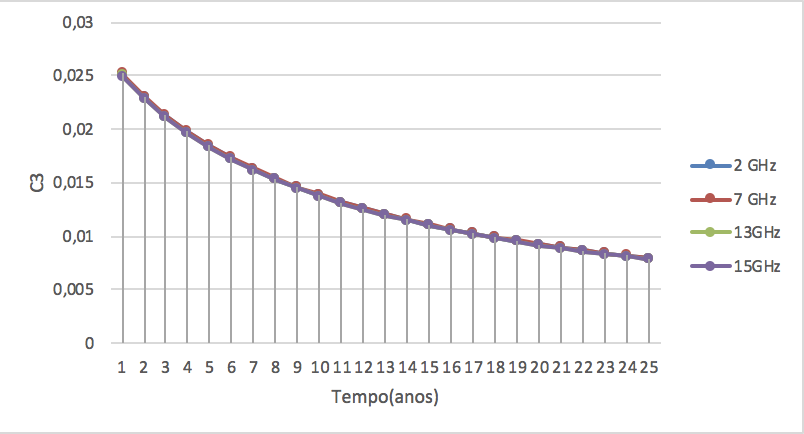
\includegraphics[scale=0.75]{custo_user.png}
\caption{Custo da chamada de 3 minutos ao longo de 25 anos para as várias frequências.}
\label{custo_user}
\end{figure}
 
 Como se pode verificar no gráfico acima representado, os custos apresentam valores muito semelhantes quer no primeiro ano, quer ao longo dos 25 anos. No entanto o menor valor de custo pertence a frequência de 15 GHz, sendo esta a escolhida para a realização do projeto.
 
\section{Especificações finais do projeto}
\begin{table}[H]
\centering
\begin{tabular}{|c|c|}
\hline
Descrição da ligação & Bidirecional entre Montijo e Fontanelas\\
Nº máximo de canais telefónicos & 120 \\
Débito Binário & 8 Mbit/s \\
Modulação & 8-PSK\\
Frequência da Portadora & 15 GHz\\
Largura de Banda & 3.5 MHz\\
Fator excesso de banda & 0.31\\
Tipo de Repetidor & Ativo\\
Localização primeira antena & Montijo (38º42'43''N;8º58'10''W)\\
Antena Parabólica Montijo & 4.5m de diâmetro\\
Azimute Montijo-Serra de Sintra & 58.3155º \\
Ângulo de fogo Montijo-Serra de Sintra & -0.34461º\\
Localização do repetidor & 38º47'33''N;9º22'38''W \\
Antena Parabólica Serra de Sintra & 4.5m de diâmetro\\
Azimute Serra de Sintra-Montijo & 258.7038º \\
Ângulo de fogo Serra de Sintra-Montijo & 0.59038\\
Azimute Serra de Sintra-Fontanelas & -137.8252º $\Leftrightarrow$ 222.1748º\\
Ângulo de fogo Serra de Sintra-Fontanelas & -1.19868º\\
Localização da segunda antena & Fontanelas(38º50'55''N;9º26'21''W )\\
Antena Parabólica Fontanelas & 4.5m de diâmetro\\
Azimute Fontanelas-Serra de Sintra & 402.1215 $\Leftrightarrow$ 42.1215\\
Ângulo de fogo Fontanelas-Serra de Sintra & 1.25692\\
\hline
\end{tabular}
\caption{Especificações da ligação por Feixes Hertzianos Digitais parte 1.}
\end{table}
\begin{table}[H]
\centering
\begin{tabular}{|c|c|}
\hline
Torre auto-suportada Montijo & 30m\\
Torre auto-suportada Serra de Sintra & 30m\\
Torre auto-suportada Fontanelas & 20m\\
Rendimento das antenas parabólicas & 0.5\\
Fator de Ruído do recetor & 8.5 dB\\
Potência do emissor & -5.66211 dBW\\
Tipo de Guias & Elípticos\\
Comprimento dos guias & 10m\\
Margem de segurança da ligação & \\
 Troço 1 & 7.2981 dB\\
 Troço 2 & 48.5089\\
Margem Crítica & \\
Troço 1 & 7.2981 dB\\
Troço 2 & 50.1769 dB\\
\hline
\end{tabular}
\caption{Especificações da ligação por Feixes Hertzianos Digitais parte 2.}
\end{table}


 
\section{Conclusão}
A execução do presente trabalho permitiu ter noção do grau de dificuldade da projeção de uma ligação de feixes hertzianos entre duas localizações com um obstáculo no caminho. Dada a complexidade e diversidade de fatores a ter em conta para a realização do projeto, as ferramentas disponibilizadas para a realização do projeto \textit{script Google Maps} para retirar o perfil e o \textit{Feixer} para determinar os caraterísticas da ligação de uma forma mais simples, simplificaram muito o trabalho a realizar. A análise de custos serviu para tomarmos conhecimento dos custos associados não só aos equipamentos e estruturas, como também às frequências e larguras de banda utilizadas para este tipo de projetos. Exemplificou ainda a abordagem a ter em consideração para tentar reduzir o custo para o utilizador ao longo do tempo.  
\pagebreak
\section{Anexos}


\begin{figure}[H]
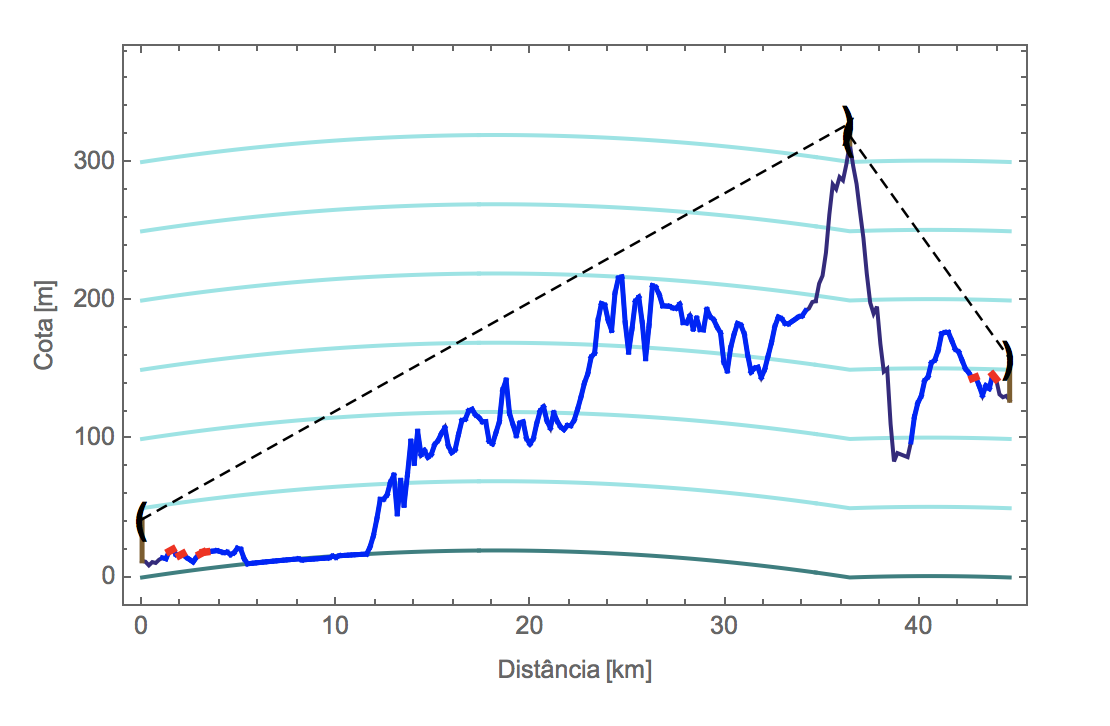
\includegraphics[scale=0.65]{reflexoes.png}
\centering
\caption{Reflexões ao longo do percurso.}
\label{reflexoes}
\end{figure}

\begin{figure}[H]
\centering
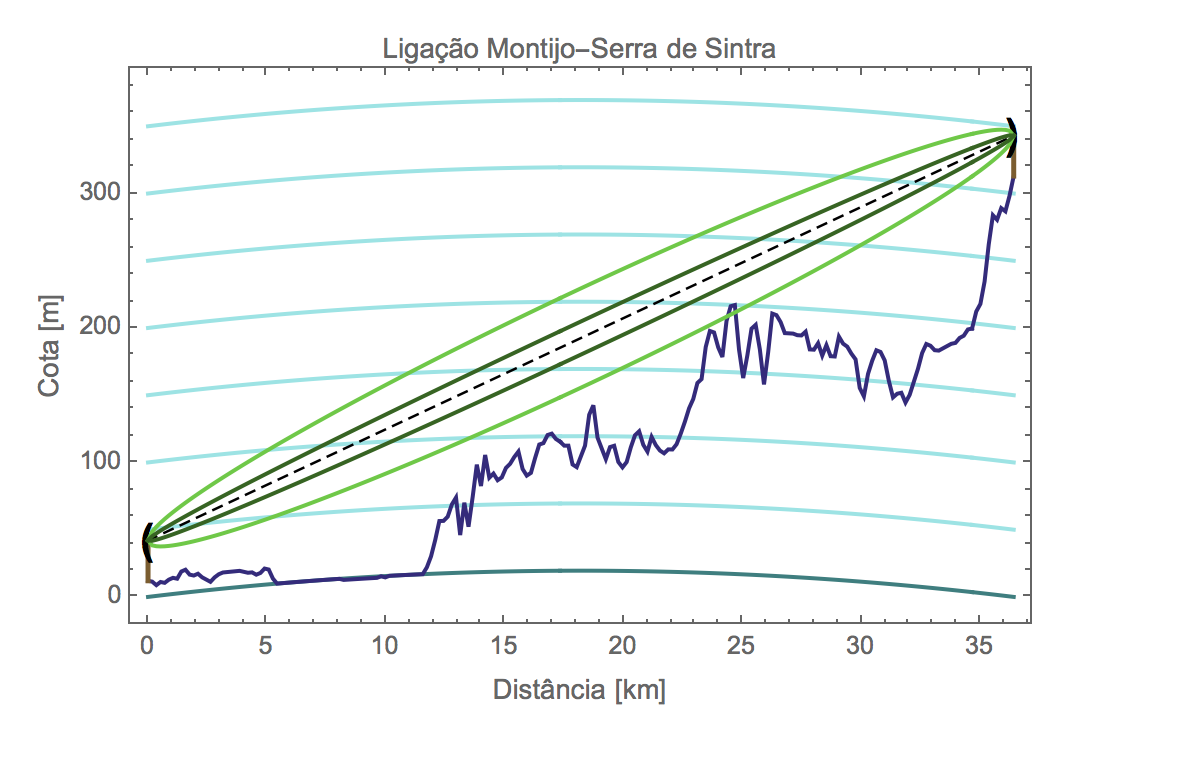
\includegraphics[scale=0.65]{perfil1.png}
\caption{Perfil da ligação Montijo-Serra de Sintra(troço 1).}
\label{perfil1}
\end{figure}

\begin{figure}[H]
\centering
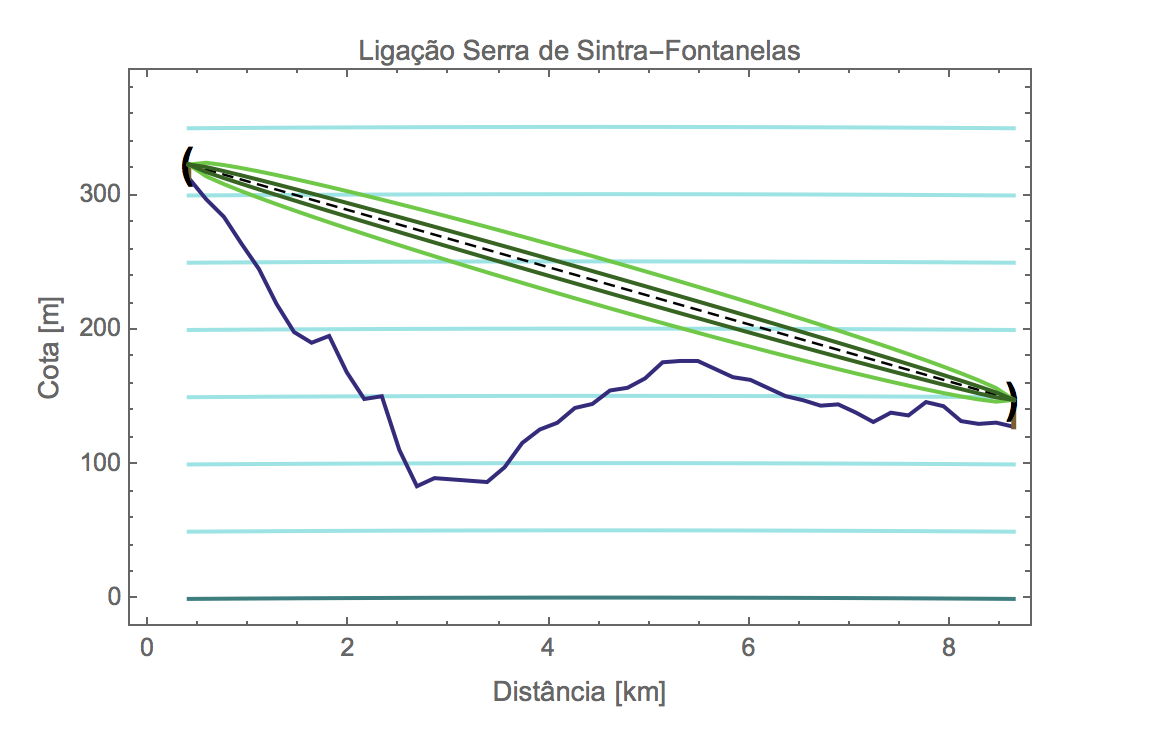
\includegraphics[scale=0.65]{perfil2.png}
\caption{Perfil da ligação Serra de Sintra-Fontanelas(troço 2).}
\label{perfil2}
\end{figure}
\begin{figure}[H]
\centering
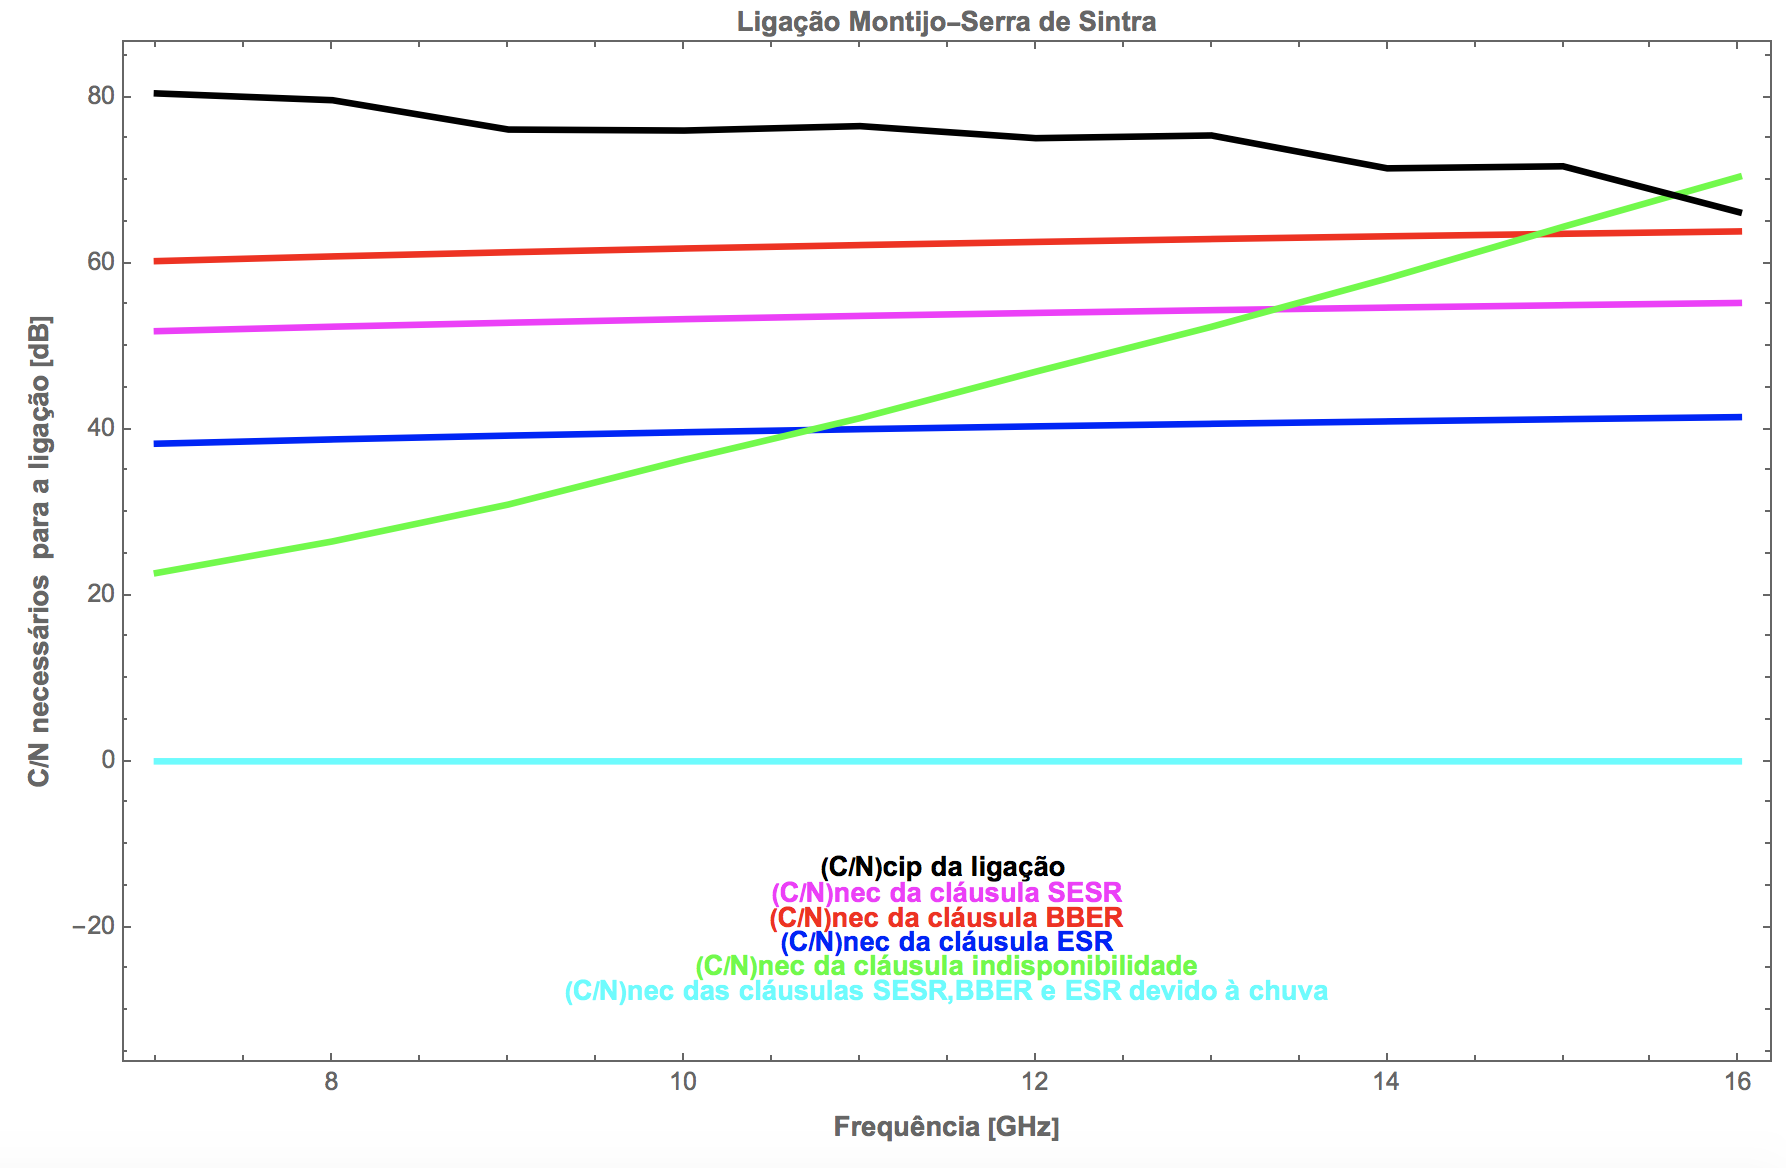
\includegraphics[scale=0.4]{cn_m_s.png}
\caption{Relação $\frac{C}{N}$ roço 1 e modulação 8-PSK com frequência 15 GHz.}
\end{figure}

\begin{figure}[H]
\centering
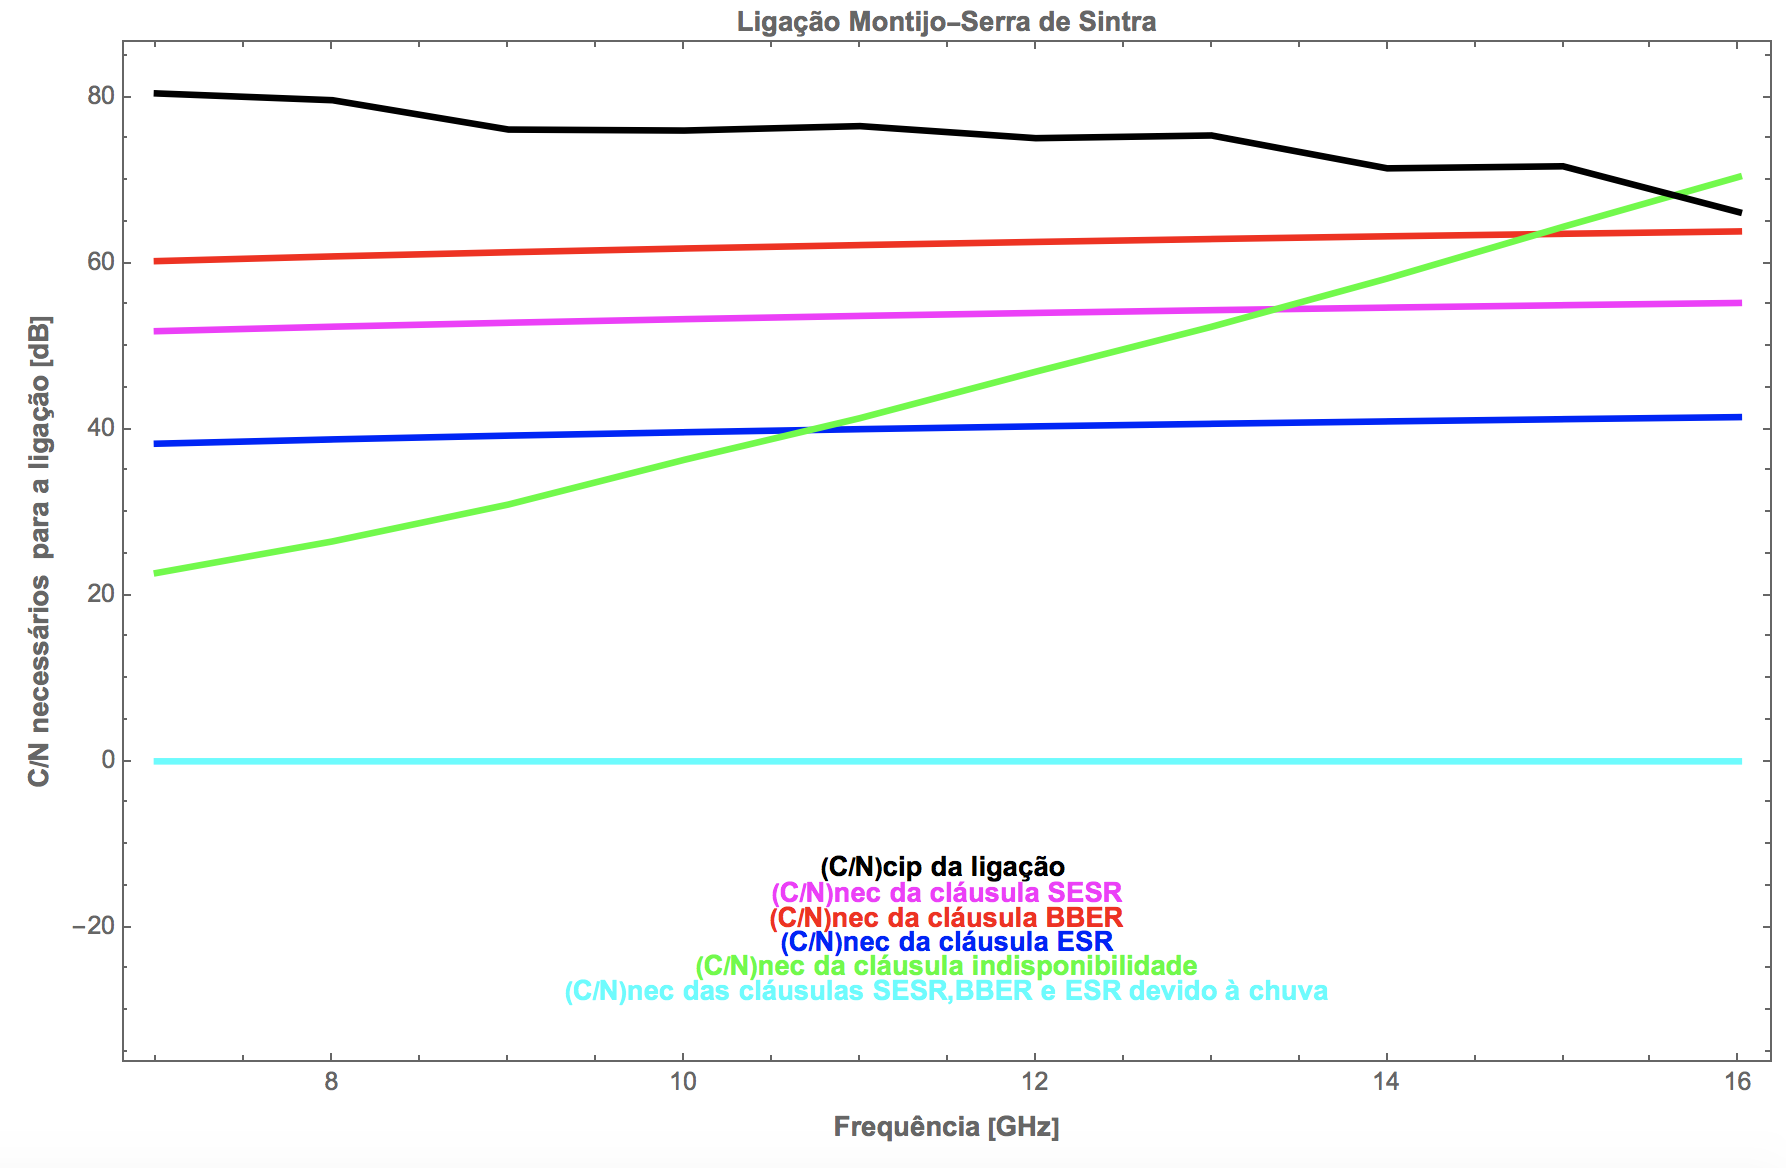
\includegraphics[scale=0.4]{cn_m_s.png}
\caption{Margem crítica para troço 1 e modulação 8-PSK com frequência 15 GHz.}
\end{figure}

\begin{figure}[H]
\centering
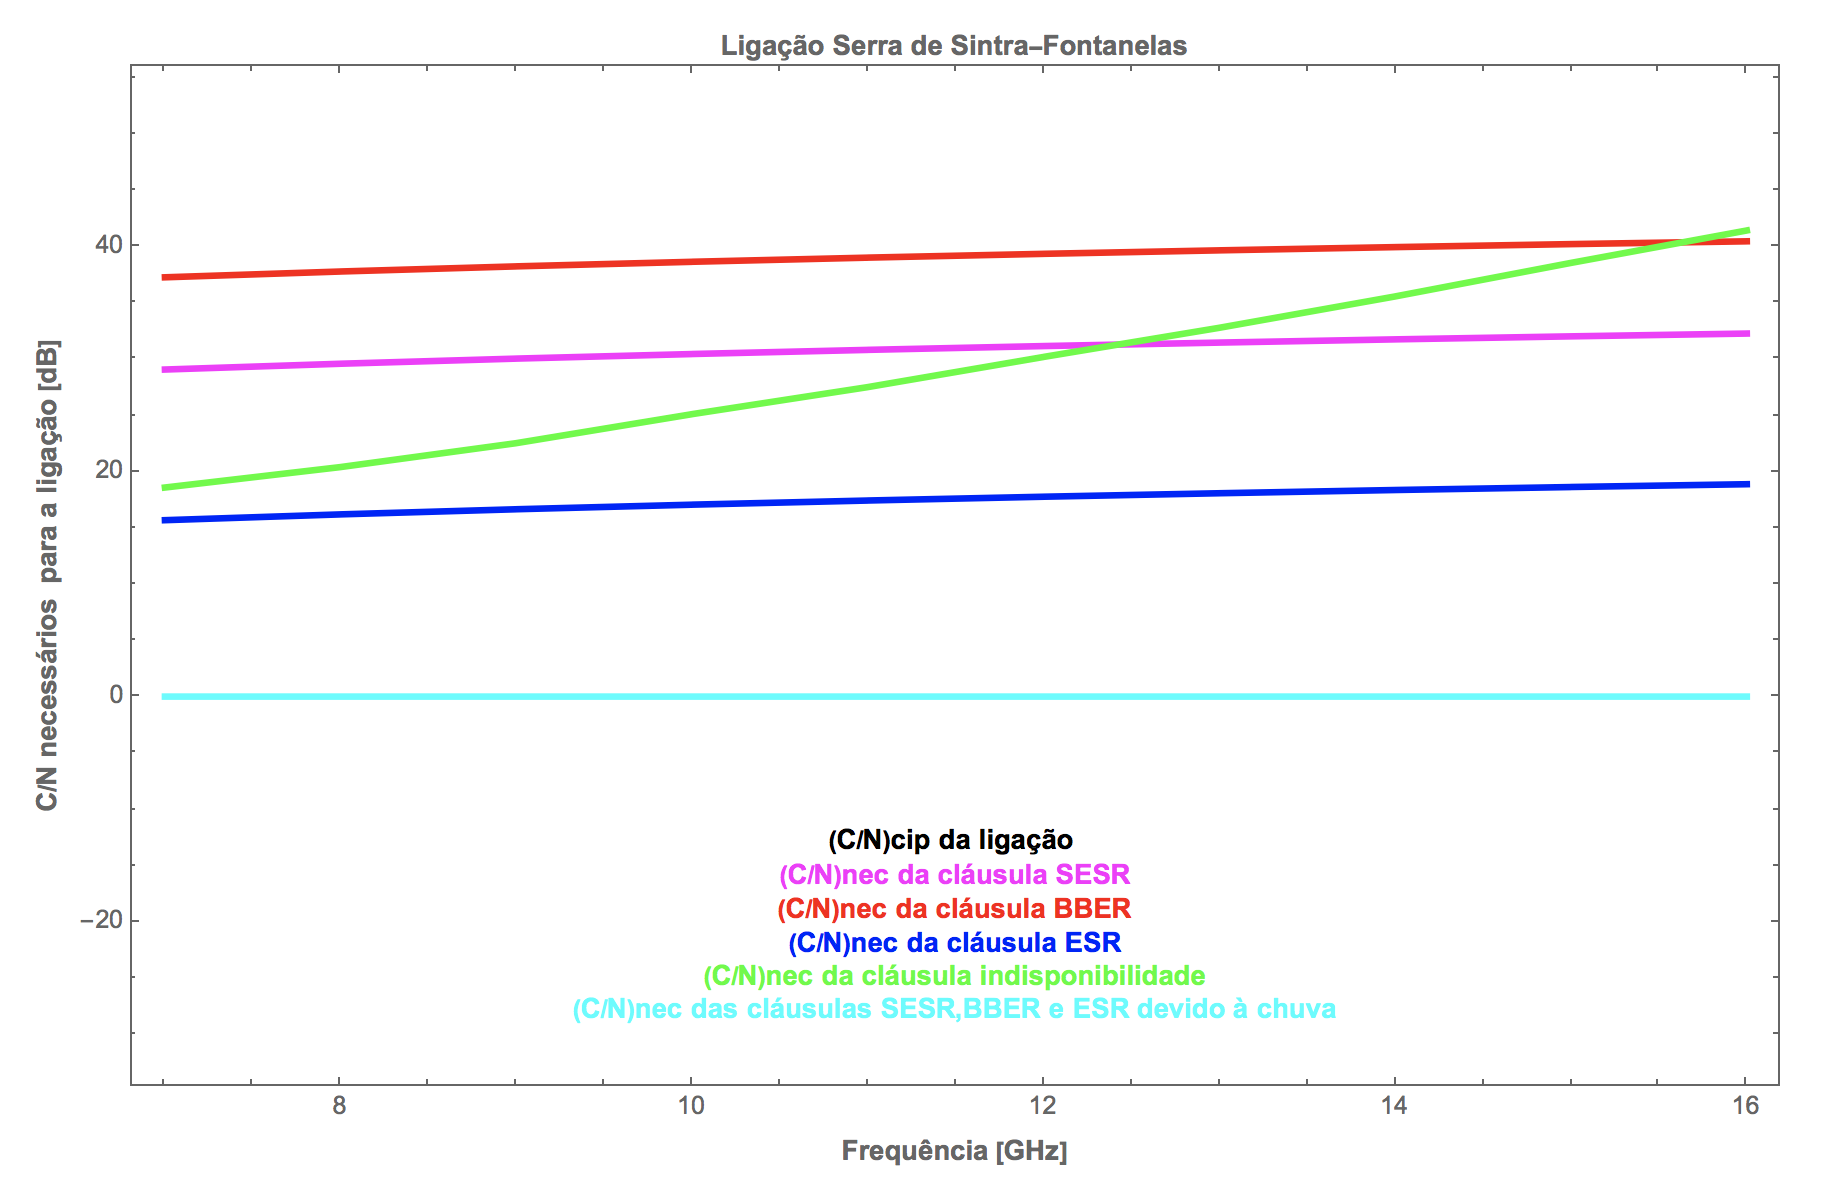
\includegraphics[scale=0.4]{cn_s_f.png}
\caption{Relação $\frac{C}{N}$ para troço 2 e modulação 8-PSK com frequência 15 GHz.}
\end{figure}

\begin{figure}[H]
\centering
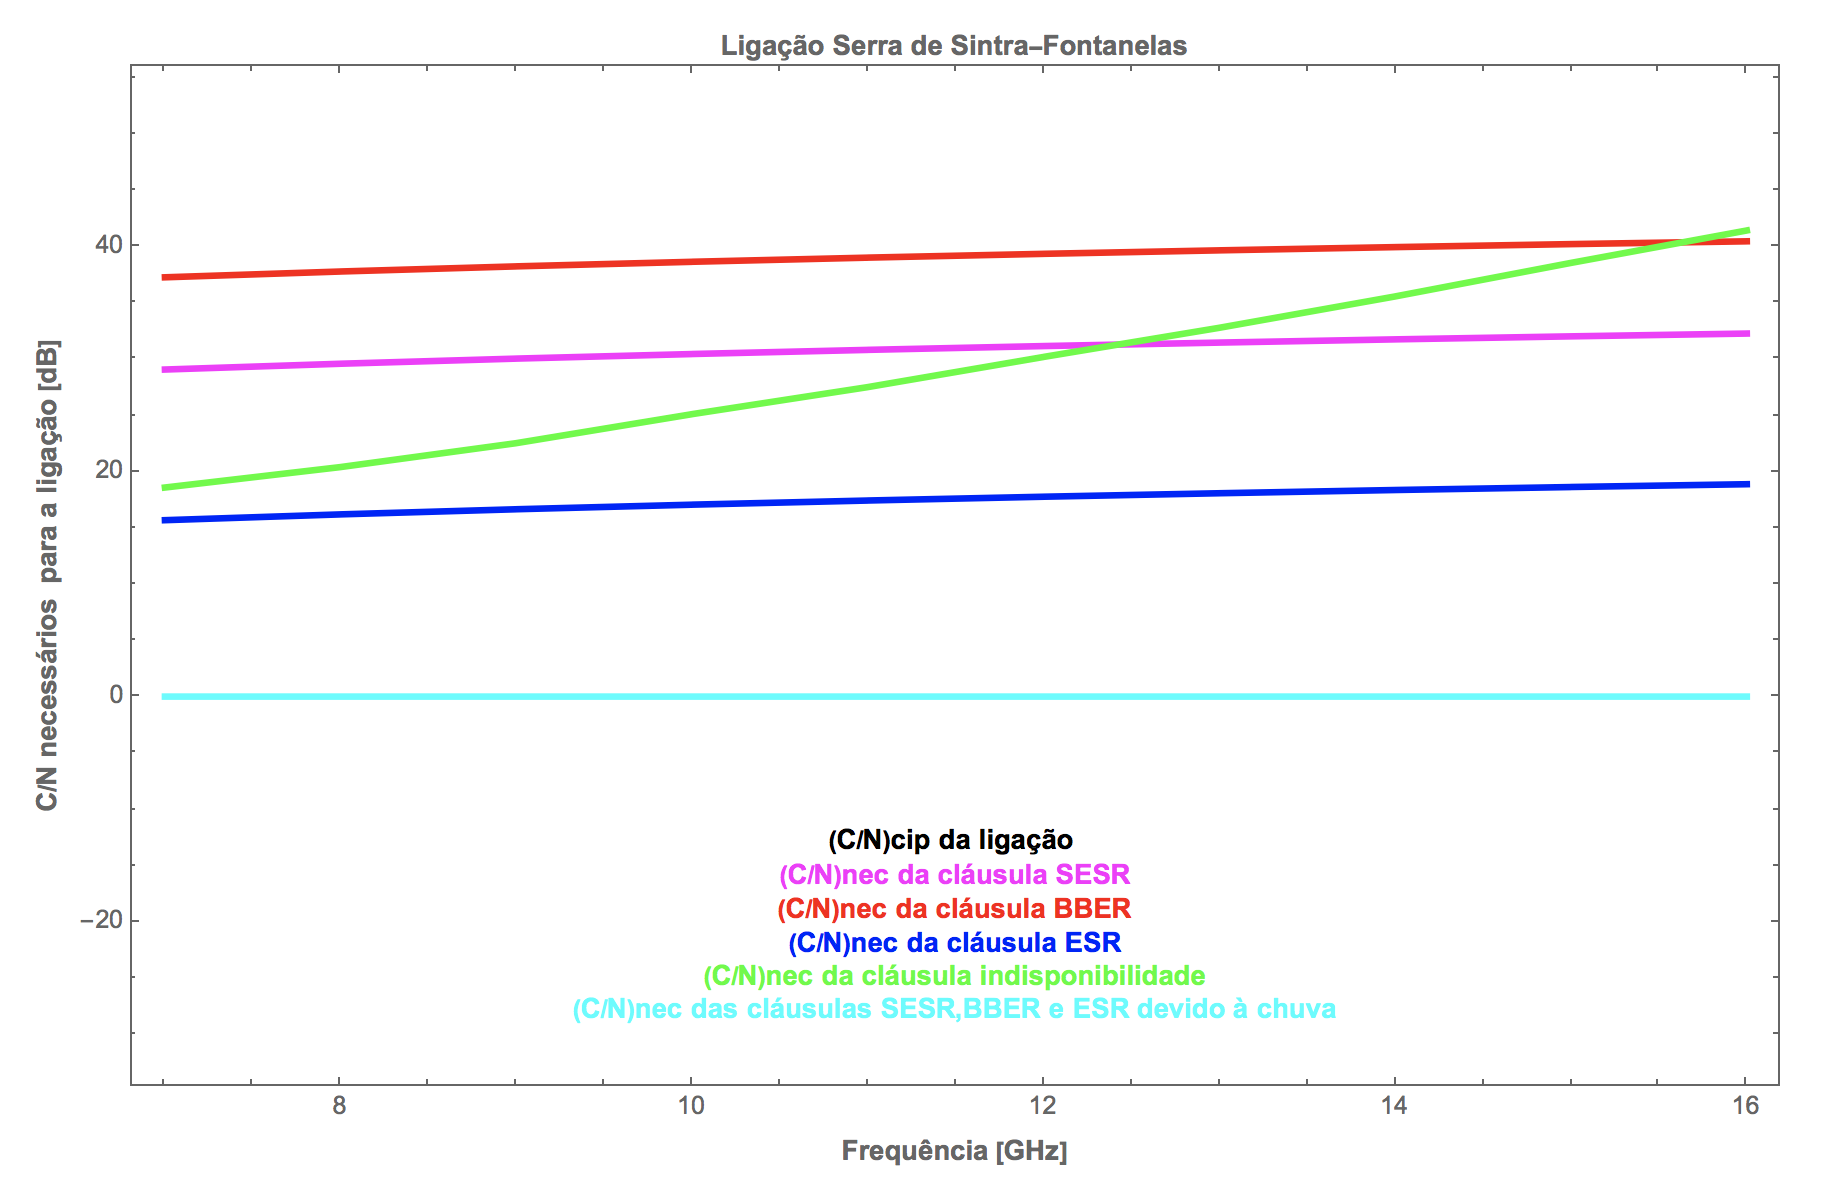
\includegraphics[scale=0.4]{cn_s_f.png}
\caption{Margem crítica para troço 2 e modulação 8-PSK com frequência 15 GHz.}
\end{figure}
 
\pagebreak
%\input{desenvolvimento}
%\pagebreak
%\input{conclusao}
%\pagebreak
%\bibliographystyle{ieeetr}
%\bibliography{bibliography}
\end{document}      
